% begin module tangents-alternative-form
\begin{frame}
\begin{columns}[c]
\column{.45\textwidth}
\psset{xunit=0.8cm, yunit=0.8cm}
\begin{pspicture}(-5, -5)(5,5) 
\psframe*[linecolor=white](-5,-5)(5,5) 
\psaxes[ticks=none, labels=none]{<->}(0,0)(-1,-1.5)(5.4,4.6)
%Function formula: -11/8+5/18 ((x) ((x) (x)))-1/81 ((x) ((x) ((x) (x))))-73/36 ((x) (x))+43/8 (x) 
\psplot[linecolor=red, plotpoints=1000]{0}{5}{x 5.375 mul x x mul -2.02778 mul add x x mul x mul x mul -0.0123457 mul add x x mul x mul 0.277778 mul add -1.375 add }

\uncover<1,11->{
\psline[linecolor=blue](0, -0.935185185)(1.531304348, 4.5)
\psFullDotBlack{0.5}{0.839506173}
}

\rput[rb] (0.6,0.92){\tiny$P=(a, f(a))$}
\rput[t](0.5, -0.1){\tiny$a$}
\psline(0.5,0.1)(0.5,0)
\uncover<2-10>{
\psline[linestyle=dashed](0.5, 0)(0.5, 0.839506173)
}

\uncover<10>{
\psline[linecolor=blue](0, -0.558641975)(1.809050773, 4.5)
\psFullDotBlack{1}{2.237654321}
\psline[linestyle=dashed](1, 0)(1, 2.237654321)
\psline(0.5, 0.839506173)(1,0.839506173) (1, 2.237654321)
\rput[t](1, -0.1){\tiny$a+h$}
\rput[l](1.1, 1.5){\tiny$f(a+h)-f(a)$}
\rput[t](0.75, 0.82){\tiny$h$}
\rput[b](1, 4){\tiny $Q=(a+h,f(a+h))$}
\psline[linestyle=dotted]{->}(1,3.9)(1, 2.237654321)
}

\uncover<9>{
\psline[linecolor=blue](0, -0.240741)(2.19429, 4.5)
\psFullDotBlack{1.5}{3}
\psline[linestyle=dashed](1.5, 0)(1.5, 3)
\psline(0.5, 0.839506173)(1.5,0.839506173) (1.5, 3)
\rput[t](1.5, -0.1){\tiny$a+h$}
\rput[l](1.6, 1.9){\tiny$f(a+h)-f(a)$}
\rput[t](1, 0.82){\tiny$h$}
\rput[b](1.5, 4){\tiny $Q=(a+h,f(a+h))$}
\psline[linestyle=dotted]{->}(1.5,3.9)(1.5, 3)
}

\uncover<8>{
\psline[linecolor=blue](0, 0.0231481)(2.74197, 4.5)
\psFullDotBlack{2}{3.28858}
\psline[linestyle=dashed](2, 0)(2, 3.28858)
\psline(0.5, 0.82)(2,0.839506173) (2, 3.28858)
\rput[t](2, -0.1){\tiny$a+h$}
\rput[l](2.1, 2){\tiny$f(a+h)-f(a)$}
\rput[t](1.25, 0.82){\tiny$h$}
\rput[b](2, 4){\tiny $Q=(a+h,f(a+h))$}
\psline[linestyle=dotted]{->}(2,3.9)(2, 3.28858)
}

\uncover<7>{
\psline[linecolor=blue](0, 0.237654)(3.54103, 4.5)
\psFullDotBlack{2.5}{3.24691}
\psline[linestyle=dashed](2.5, 0)(2.5, 3.24691)
\psline(0.5, 0.839506173)(2.5,0.839506173) (2.5, 3.24691)
\rput[t](2.5, -0.1){\tiny$a+h$}
\rput[l](2.6, 2){\tiny$f(a+h)-f(a)$}
\rput[t](1.5, 0.82){\tiny$h$}
\rput[b](2.5, 4){\tiny $Q=(a+h,f(a+h))$}
\psline[linestyle=dotted]{->}(2.5,3.9)(2.5, 3.24691)
}

\uncover<6>{
\psline[linecolor=blue](0, 0.407407)(4.73571, 4.5)
\psFullDotBlack{3}{3}
\psline[linestyle=dashed](3, 0)(3, 3)
\psline(0.5, 0.839506173)(3,0.839506173) (3, 3)
\rput[t](3, -0.1){\tiny$a+h$}
\rput[l](3.1, 1.9){\tiny$f(a+h)-f(a)$}
\rput[t](1.75, 0.82){\tiny$h$}
\rput[b](3, 4){\tiny $Q=(a+h,f(a+h))$}
\psline[linestyle=dotted]{->}(3,3.9)(3, 3)
}

\uncover<5>{
\psline[linecolor=blue](0, 0.537037)(5, 3.56173)
\psFullDotBlack{3.5}{2.65432}
\psline[linestyle=dashed](3.5, 0)(3.5, 2.65432)
\psline(0.5, 0.839506173)(3.5,0.839506173) (3.5, 2.65432)
\rput[t](3.5, -0.1){\tiny$a+h$}
\rput[l](3.6, 1.7){\tiny$f(a+h)-f(a)$}
\rput[t](2, 0.82){\tiny$h$}
\rput[b](3.5, 4){\tiny $Q=(a+h,f(a+h))$}
\psline[linestyle=dotted]{->}(3.5,3.9)(3.5, 2.65432)
}

\uncover<2-4>{
\psline[linecolor=blue](0, 0.631173)(5, 2.71451)
\psFullDotBlack{4}{2.29784}
\psline[linestyle=dashed](4, 0)(4, 2.29784)
\psline(0.5, 0.839506173)(4,0.839506173) (4, 2.29784)
\psline[linestyle=dotted]{->}(4,3.9)(4, 2.29784)
}
\uncover<2>{
\rput[t](4, -0.1){\tiny$x$}
\rput[l](4.1, 1.5){\tiny$f(x)-f(a)$}
\rput[t](2.25, 0.82){\tiny$x-a$}
\rput[b](4, 4){\tiny $Q=(x,f(x))$}
}
\uncover<3,4>{
\rput[t](4, -0.1){\tiny$a+h$}
\rput[l](4.1, 1.5){\tiny$f(a+h)-f(a)$}
\rput[t](2.25, 0.82){\tiny$h$}
\rput[b](4, 4){\tiny $Q=(a+h,f(a+h))$}
}
\end{pspicture} 
%\ \only<handout:0| -1,12->{%
%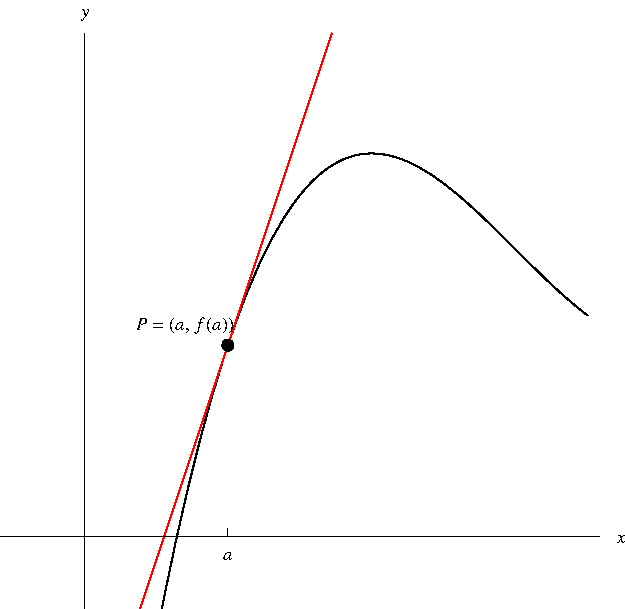
\includegraphics[height=4.5cm]{derivatives/pictures/03-01-tangent.pdf}%
%}%
%\only<handout:1| 2>{%
%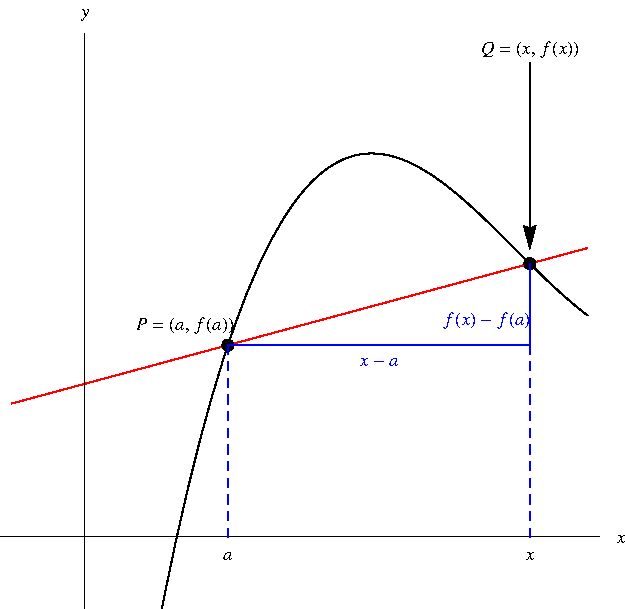
\includegraphics[height=4.5cm]{derivatives/pictures/03-01-secanta.pdf}%
%}%
%\only<handout:2-| 3-5>{%
%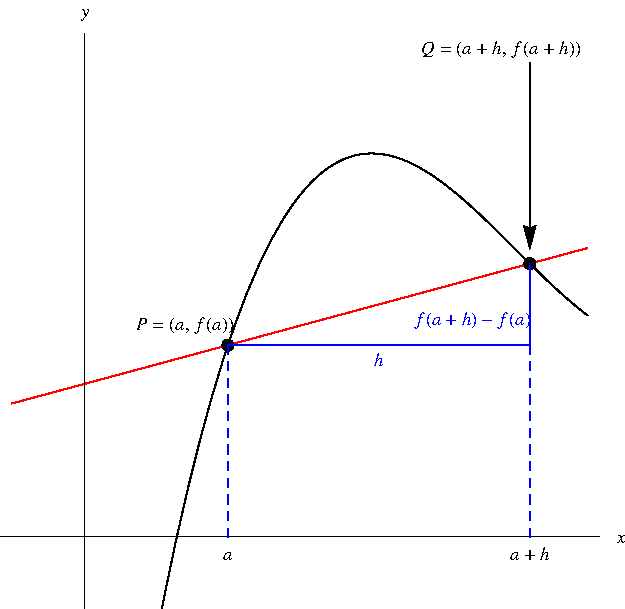
\includegraphics[height=4.5cm]{derivatives/pictures/03-01-secantha.pdf}%
%}%
%\only<handout:0| 6>{%
%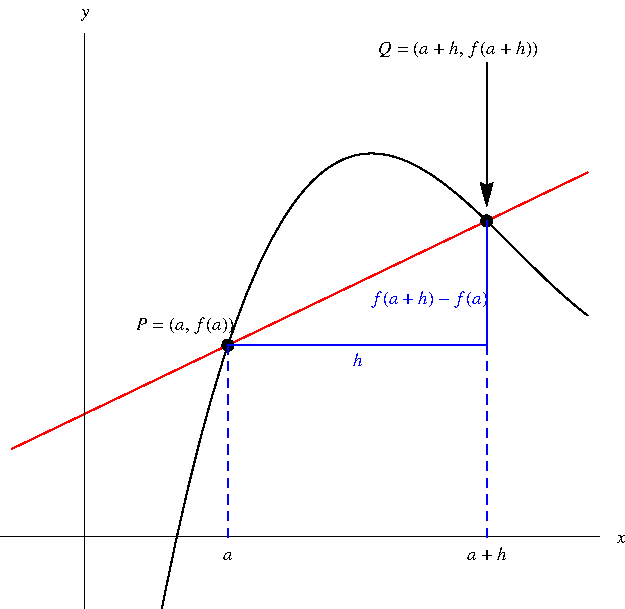
\includegraphics[height=4.5cm]{derivatives/pictures/03-01-secanthb.pdf}%
%}%
%\only<handout:0| 7>{%
%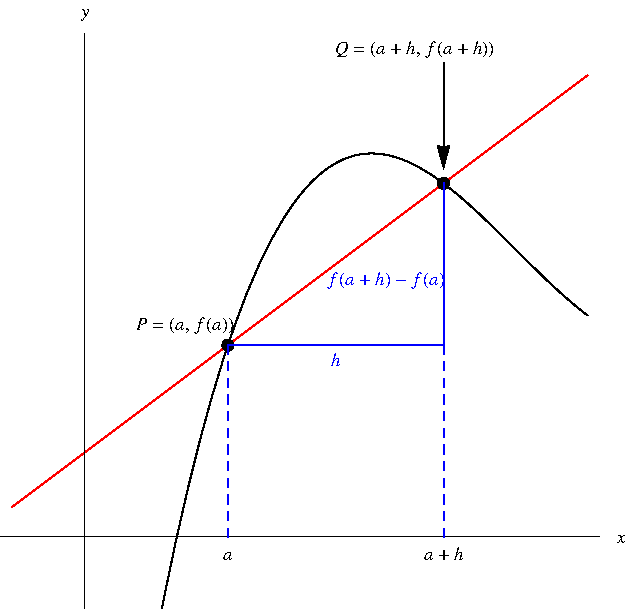
\includegraphics[height=4.5cm]{derivatives/pictures/03-01-secanthc.pdf}%
%}%
%\only<handout:0| 8>{%
%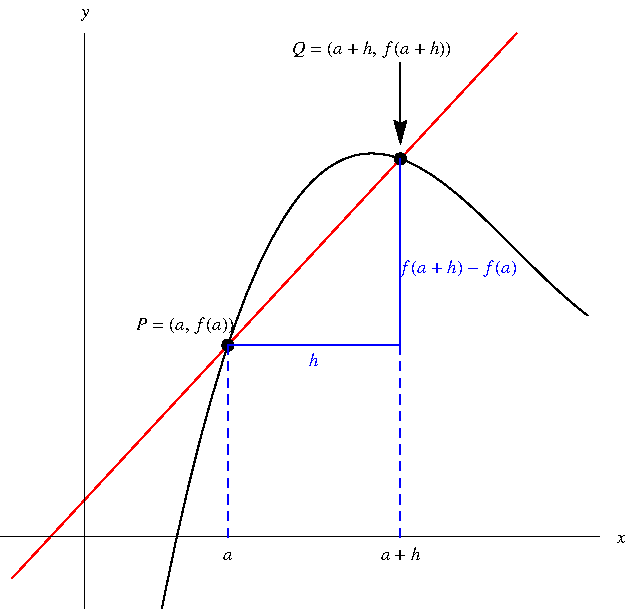
\includegraphics[height=4.5cm]{derivatives/pictures/03-01-secanthd.pdf}%
%}%
%\only<handout:0| 9>{%
%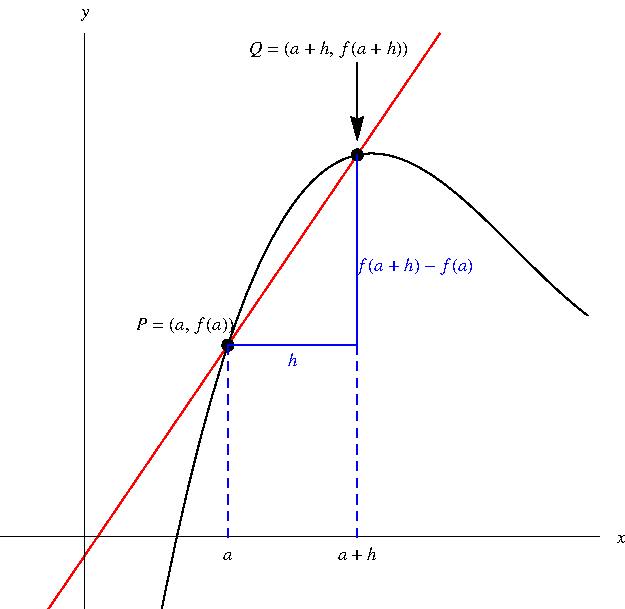
\includegraphics[height=4.5cm]{derivatives/pictures/03-01-secanthe.pdf}%
%}%
%\only<handout:0| 10>{%
%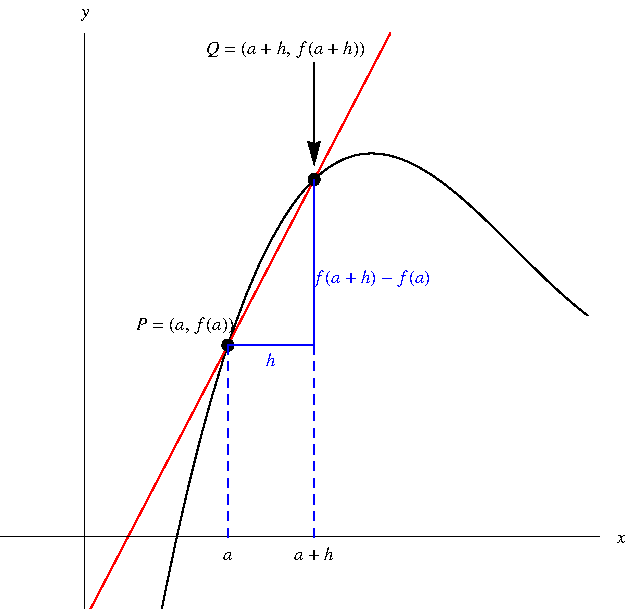
\includegraphics[height=4.5cm]{derivatives/pictures/03-01-secanthf.pdf}%
%}%
%\only<handout:0| 11>{%
%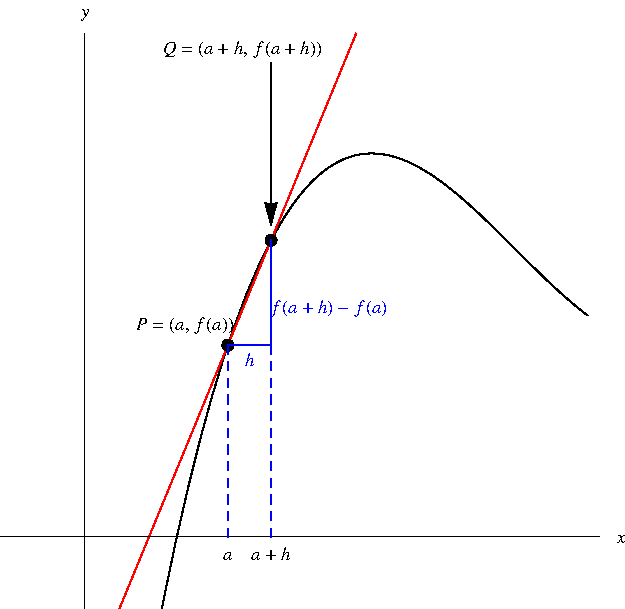
\includegraphics[height=4.5cm]{derivatives/pictures/03-01-secanthg.pdf}%
%}%
\column{.55\textwidth}
\begin{itemize}
\item<1->  There is an equivalent expression for the slope of the tangent.
\item<2->  Again let $x$ tend to $a$.
\item<handout:2-| 3->  However, think in terms of $h = x - a$.
\item<handout:2-| 4->  Then $x = a+h$ and the slope of the secant line $PQ$ is $m_{PQ} = \frac{f(a+h)-f(a)}{h}$.
\item<handout:2-| 5->  The limit can now be written in terms of the quantity $h$.
\end{itemize}
\end{columns}

\uncover<handout:2-| 12->{%
Tangent slope - equivalent expression:
\[
m = \lim_{h\rightarrow 0}\frac{f(a+h) - f(a)}{h}.
\]
}%
\end{frame}
% end module tangents-alternative-form